\subsection{Hồi quy tuyến tính đa bội}
\subsubsection{Mục đích}

Mục đích của mô hình hồi quy tuyến tính này là dự đoán giá trị tổng đơn hàng dựa trên các yêu tố giải thích khác nhau như giá trị đơn hàng, phí vận chuyển,..

\subsubsection{Kiểm tra dữ liệu có tuân theo phân phối chuẩn hay không} 

Ta cần kiểm tra xem các dữ liệu của ta có tuân theo quy luật phận phối chuẩn hay không bằng cách cho mức ý nghĩa là 5\%, ta dùng lệnh \textbf{shapiro.test()} để kiểm tra p-value. Nếu giá trị p-value > 0.05, thì cột dữ liệu đó tuân theo phân phối chuẩn và ngược lại.Thực hiện trên Rstudio ta thu được kết quả:


\begin{figure}[H]
  \centering
  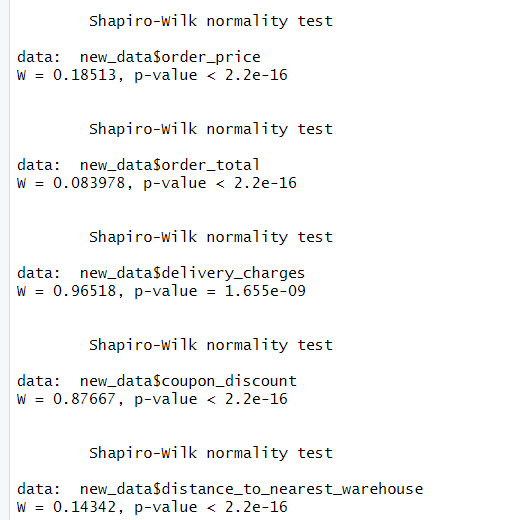
\includegraphics[width=0.5\linewidth]{graphics/5.5.0.png}
  \caption{kết quả kiểm  tra phân phối chuẩn của các biến }
\end{figure}

5 cột dữ liệu đều có p-value < 0.05, điều đó cho ta thấy cả 5 cột không tuân theo quy luật phân phối chuẩn.

Tuy dữ liệu không tuân theo quy luật phân phối chuẩn nhưng mẫu đủ lớn, ta vẫn có thể sử dụng hồi quy tuyến tính mà không cần lo ngại quá nhiều về vấn đề phân phối chuẩn của dữ liệu. Điều này dựa trên lý thuyết \textbf{Lý thuyết Giới hạn Trung tâm (Central Limit Theorem - CLT)}. 

Lý thuyết Giới hạn Trung tâm là một khái niệm quan trọng trong thống kê vì nó cho phép chúng ta làm việc với các mẫu ngẫu nhiên mà không cần phải lo lắng về phân phối gốc của dữ liệu. Nó đảm bảo rằng, khi kích thước mẫu đủ lớn, các phân tích thống kê có thể sử dụng phân phối chuẩn để thực hiện các ước lượng và kiểm định giả thuyết, ngay cả khi dữ liệu gốc không tuân theo phân phối chuẩn.
\subsubsection{Xây dựng mô hình hồi quy tuyến tính}
Trước tiên ta kiểm tra sự phụ thuộc của biến delivery\_charges vào hai biến độc lập is\_expedited\_delivery và distance\_to\_nearest\_warehouse. Ta sử dụng lệnh lm().

Kết quả phân tích trên Rstudio:
\begin{figure}[H]
  \centering
  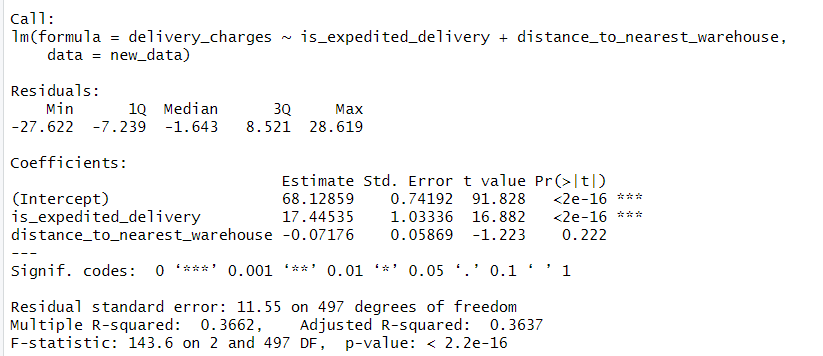
\includegraphics[width=0.7\linewidth]{graphics/5.5.1.png}
  \caption{Kết quả hồi quy tuyến tính giữa 2 biến delivery\_charges và is\_expedited\_delivery  }
\end{figure}


Với mức ý nghĩa 5\%, ta phân tích phần Coefficients (hệ số) như sau:

Định nghĩa biến $x_1$: is\_expedited\_delivery,$x_2$:distance\_to\_nearest\_warehouse, y:delivery\_charges

Cho biết hệ số của biến độc lập trong phương trình: $\beta_0= 68.12859, \beta_1= 17.44535,\\ \beta_2= -0.07176 $
 
Ta có phương trình hồi quy tuyến tính đơn giản: $y= 68.12859 + 17.44535x_1 - 0.07176x_2$

 Dựa vào bảng số liệu trên ta có:\\
 \begin{itemize}
 \item\textbf{Pr(>|t|)}: Chỉ có giá trị p-value của biến distance\_to\_nearest\_warehouse lớn hơn 0.05(0.222>0.05), cho thấy biến distance\_to\_nearest\_warehouse không có ý nghĩa thống kê trong mô hình này. Có thể xem như hai biến delivery\_charges và distance\_to\_nearest\_warehouse độc lập với nhau.
\item\textbf{Multiple R-squared}: 0.3662, cho thấy mô hình giải thích được 36.62\% biến động của delivery\_charges.
 \end{itemize}

 Mô hình hồi quy này chỉ ra rằng việc giao hàng nhanh \textbf{(is\_expedited\_delivery)} có ảnh hưởng đáng kể và có ý nghĩa thống kê đến chi phí giao hàng \textbf{(delivery\_charges)}. Mặc dù mô hình giải thích được \textbf{36.62\%} biến động của chi phí giao hàng, điều này cho thấy vẫn còn nhiều yếu tố khác cần được xem xét để giải thích toàn bộ biến động của chi phí giao hàng.

Trên thực tế tổng giá trị đơn hàng phụ thuộc vào tổng giá trị mặt hàng, chi phí vận chuyển, mã giảm giá, khoảng cách đến kho hàng gần nhất,....Vậy nên ta chọn biến \textbf{order\_total} làm biến phụ thuộc vào các biến độc lập \textbf{order\_price, delivery\_charges},\textbf{coupon\_discount} và \textbf{distance\_to\_nearest\_warehouse}.

Ta xét khi có các biến ngoại lai. Hồi quy tuyến tính mô hình trên ta có được:
\begin{figure}[H]
  \centering
  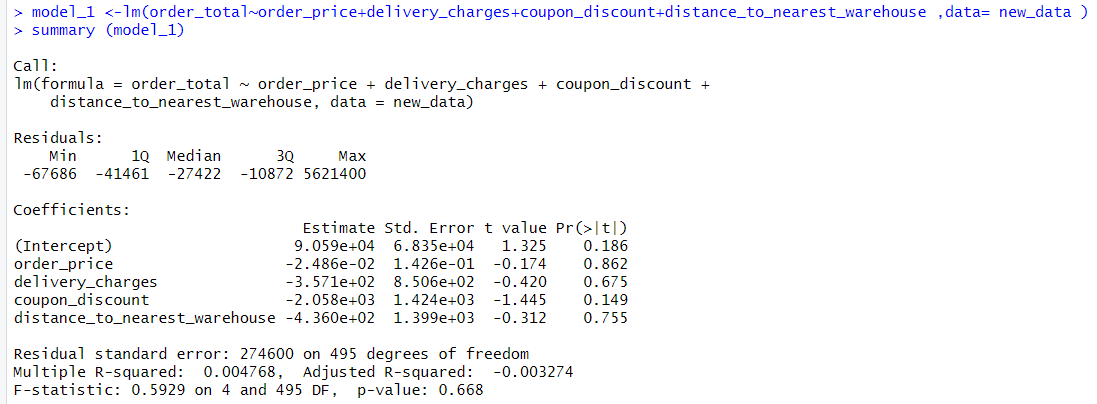
\includegraphics[width=0.7\linewidth]{graphics/5.5.2.png}
  \caption{Kết quả hồi quy tuyến tính mô hình 1 }
\end{figure}

Dựa trên kết qủa từ hàm \textbf{summary(model\_1)} ta rút ra nhận xét sau:
\begin{itemize}
\item \textbf{(Intercept)}: Khi tất cả các biến độc lập bằng 0, giá trị trung bình của order\_total là 90590. Tuy nhiên, giá trị p-value là 0.186, không có ý nghĩa thống kê.
\item \textbf{order\_price}: Hệ số ước lượng là -0.02486, và p-value là 0.862, không có ý nghĩa thống kê.
\item \textbf{delivery\_charges}: Hệ số ước lượng là -357.1, và p-value là 0.675, không có ý nghĩa thống kê.
\item \textbf{coupon\_discount}: Hệ số ước lượng là -2058.0, và p-value là 0.149, không có ý nghĩa thống kê.
\item \textbf{distance\_to\_nearest\_warehouse}: Hệ số ước lượng là -436.0, và p-value là 0.755, không có ý nghĩa thống kê.
\item\textbf{Multiple R-squared}: 0.004768, chỉ ra rằng mô hình chỉ giải thích được 0.4768\% biến động của order\_total.
\item\textbf{F-statistic}: 0.5929, với p-value là 0.668, cho thấy mô hình tổng thể không có ý nghĩa thống kê
\end{itemize}

Mô hình hồi quy model\_1 không phù hợp tốt với dữ liệu của bạn bởi vì:
\begin{itemize}
\item Các biến độc lập đều không có ý nghĩa thống kê ($p-value > 0.05$).
\item Chỉ số \textbf{R-squared} rất thấp, cho thấy mô hình không giải thích được biến động của order\_total.
\item\textbf{F-statistic} không có ý nghĩa thống kê, gợi ý rằng mô hình tổng thể không phù hợp.
\end{itemize}

Tiếp theo ta xét tiếp khi bỏ các giá trị ngoại lai

Hồi quy trên Rstudio ta có được:
\begin{figure}[H]
  \centering
  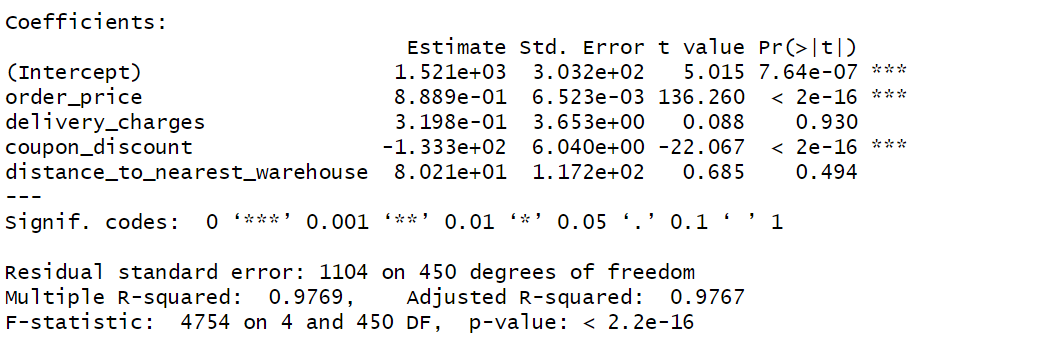
\includegraphics[width=0.7\linewidth]{graphics/5.5.3.png}
  \caption{Kết quả hồi quy tuyến tính mô hình 2 }
\end{figure} 

Dựa trên kết quả từ hàm \textbf{summary(model\_2)}, ta có thể rút ra các nhận xét:

Với mức ý nghĩa 5\%, ta phân tích phần Coeficients(hệ số) như sau:

Định nghĩa các biến:  y: order\_total, $x_1$: order\_price, $x_2$: delivery\_charges, $x_3$: coupon\_discount, $x_4$: distance\_to\_nearest\_warehouse.

Cho các hệ số của từng biến độc lập trong phương trình : $\beta_0= 1450, \beta_1= 0.8887, \\\beta_2= 1.132, \beta_3= -133.9, \beta_4= 103.1$ Ta có phương trình hồi quy: 

 \hspace{25mm}$y= 1450 + 0.8887x_1 + 1.132x_2 - 133.9x_3 + 103.1x_4$

Ý nghĩa của hệ số hồi quy:
\begin{itemize}
\item\textbf{(Intercept)}: Khi tất cả các biến độc lập bằng 0, giá trị trung bình của order\_total là 1450.0. Giá trị p-value rất nhỏ (1.57e-05), có ý nghĩa thống kê.
\item\textbf{order\_price}: Hệ số ước lượng là 0.8887, và p-value rất nhỏ (< 2e-16), có ý nghĩa thống kê mạnh mẽ. Mỗi đơn vị tăng của order\_price dẫn đến order\_total tăng trung bình 0.8887 đơn vị, giữ nguyên các yếu tố khác.\\
\item\textbf{delivery\_charges}: Hệ số ước lượng là 1.132, và p-value là 0.776, không có ý nghĩa thống kê.
\item\textbf{coupon\_discount}: Hệ số ước lượng là -133.9, và p-value rất nhỏ (< 2e-16), có ý nghĩa thống kê mạnh mẽ. Mỗi đơn vị tăng của coupon\_discount dẫn đến order\_total giảm trung bình 133.9 đơn vị, giữ nguyên các yếu tố khác.
\item\textbf{distance\_to\_nearest\_warehouse}: Hệ số ước lượng là 103.1, và p-value là 0.399, không có ý nghĩa thống kê.
\end{itemize}

Chỉ số đo lường của mô hình:

\begin{itemize}
\item\textbf{Multiple R-squared}: 0.9765, cho thấy mô hình giải thích được 97.65\% biến động của order\_total.
\item\textbf{F-statistic}: 4534, với p-value < 2.2e-16, cho thấy mô hình tổng thể có ý nghĩa thống kê mạnh mẽ.
\end{itemize}

Từ 2 mô hình trên ta có thể thấy được rằng giá trị ngoại lai ảnh hưởng đến hồi quy tuyến tính như thế nào. Các giá trị ngoại lai có thể làm suy yếu mô hình hồi quy tuyến tính, làm giảm khả năng giải thích của mô hình và làm sai lệch các hệ số ước lượng. Sau khi xử lý ngoại lai, mô hình có sự cải thiện rõ rệt, với giá trị R-squared cao hơn và các biến có ý nghĩa thống kê tốt hơn. Việc loại bỏ các ngoại lai giúp làm sạch dữ liệu và cải thiện độ chính xác của mô hình.

Qua mô hình 2 ta thấy có hai biến là biến \textbf{order\_price} và \textbf{coupon\_discout} là phù hợp (p-value<0.05), vì thế nên ta loại bỏ hai biến còn lại ra khỏi mô hình.

Loại bỏ hai biến \textbf{delivery\_charges} và \textbf{distance\_to\_nearest\_warehouse}, giữ lại biến có ý nghĩa là \textbf{order\_price} và \textbf{coupon\_discount}.

Từ đó ta có mô hình 3 : $y= \beta_0 + \beta_1x_1 + \beta_2x_2$ với y: order\_total, $x_1$: order\_price, $x_2$: coupon\_discount.

Ta tiếp sử dụng Rstudio để phân tích mô hình 3
\begin{figure}[H]
  \centering
  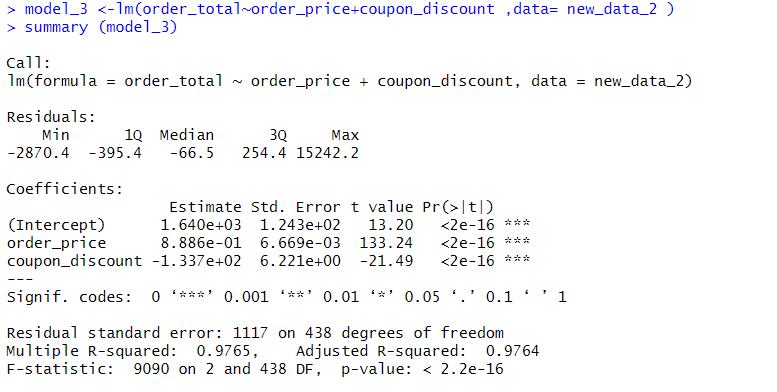
\includegraphics[width=0.7\linewidth]{graphics/5.5.4.png}
  \caption{Kết quả hồi quy tuyến tính mô hình 3 }
\end{figure}

Với mức ý nghĩa 5\% ta có phương trình: $y= 1640 + 0.8886x_1 - 133.7 x_2$

Ý nghĩa của hệ số hồi quy:
\begin{itemize}
\item\textbf{(Intercept)}: Hệ số chặn (Intercept) là 1640, có ý nghĩa thống kê mạnh (p-value < 0.001).
\item\textbf{order\_price}: Hệ số của order\_price là 0.8886, có ý nghĩa thống kê mạnh với p-value rất nhỏ (< 0.001). Điều này cho thấy mối quan hệ tích cực giữa order\_price và order\_total, tức là khi giá trị đơn hàng tăng, tổng giá trị đơn hàng cũng tăng.
\item\textbf{coupon\_discount}: Hệ số của coupon\_discount là -133.7, có ý nghĩa thống kê mạnh với p-value < 0.001. Mối quan hệ này cho thấy khi mức giảm giá (coupon) tăng lên, tổng giá trị đơn hàng giảm đi.
\end{itemize}

Chỉ số đo lường mô hình:

\begin{itemize}
\item\textbf{Multiple R-squared}: 0.9765, cho thấy mô hình giải thích được 97.65\% biến động của order\_total.
\item\textbf{F-statistic}: 9090, với p-value < 2.2e-16, cho thấy mô hình tổng thể có ý nghĩa thống kê mạnh mẽ.
\end{itemize}

Mô hình 3 có hiệu quả rất cao trong việc giải thích sự biến thiên của \textbf{order\_total}, với \textbf{R-squared} lên đến \textbf{97.65\%}. Các biến \textbf{order\_price} và \textbf{coupon\_discount} là những yếu tố quan trọng và có ảnh hưởng rõ rệt đến tổng giá trị đơn hàng. Việc loại bỏ các biến không quan trọng như \textbf{delivery\_charges} và \textbf{distance\_to\_nearest\_warehouse} giúp đơn giản hóa mô hình mà vẫn giữ được khả năng dự đoán chính xác.

\subsubsection{Kiểm định lại mô hình hồi quy tuyến tính}
Tiếp tục kiểm định, ta xác định khoảng tin cậy cho hệ số với mức ý nghĩa 5\%\ bằng lệnh \textbf{confint(model\_3)}:
\begin{figure}[H]
  \centering
  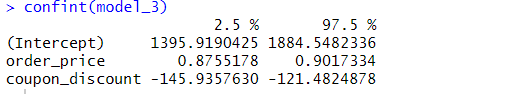
\includegraphics[width=0.7\linewidth]{graphics/5.5.5.png}
  \caption{Kiểm định khoảng tin cậy hệ số mô hình 3 }
\end{figure}

Ta thấy các hệ số $\beta_0= 1640\in(1395.91904; 1884.5482), \beta_1= 0.8886\in(.8755;0.9017),\\ \beta_2= -133.7\in(-145.9358 -121.4825)$

Kiểm định bằng phương pháp so sánh với giá trị thực tế:

Ta tiến hành thay các giá trị $x_1$, $x_2$ vào phương trình(ở mô hình 3): $y= 1640 + 0.8886x_1 - 133.7 x_2$ sau đó so sánh với giá trị order\_total trong bảng. Ta sử dụng Rstudio để thực hiện thao tác trên:

\begin{figure}[H]
  \centering
  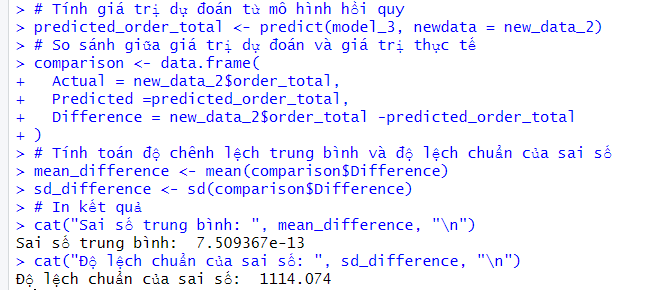
\includegraphics[width=0.5\linewidth]{graphics/5.5.7.png}
  \caption{So sánh giá trị hồi quy với giá trị thực tế }
\end{figure}

Ta sử dụng lệnh predict để tiến hành thay các giá trị vào phương trình. Sau khi tiến hành so sánh ta thu được hai thống số là:
\begin{itemize}
  \item Sai số trung bình : 7.509367e-13. Kết quả rất gần 0 (7.509367e-13 \approx 0), cho thấy mô hình không bị lệch. Sai số trung bình nhỏ này phản ánh rằng giá trị dự đoán trung bình khá khớp với giá trị thực tế.
  \item Độ lệch chuẩn của sai số: 1114.074. Độ lệch chuẩn là 1114.074, khá nhỏ so với một số giá trị order\_total thực tế (ví dụ: hàng chục ngàn). Điều này chỉ ra rằng các dự đoán của mô hình có mức độ ổn định tương đối.
\end{itemize}

Kiểm định phân phối chuẩn của phần dư bằng Shapiro-Wilk:

Giả thuyết đặt ra:
\begin{itemize}
  \item\textbf{Giả thuyết H0}: Phần dư của mô hình hồi quy tuân theo phân phối chuẩn.
  \item\textbf{Giả thuyết H1}: Phần dư của mô hình hồi quy không tuân theo phân phối chuẩn.
  \item Nếu p-value ≥ a (thường chọn a = 0.05): Không đủ bằng chứng bác bỏ H₀ \rightarrow Phần dư có thể coi là tuân theo phân phối chuẩn.
  \item Nếu p-value < a: Bác bỏ H0 \leftarrow Phần dư không tuân theo phân phối chuẩn.
\end{itemize}

\begin{figure}[H]
  \centering
  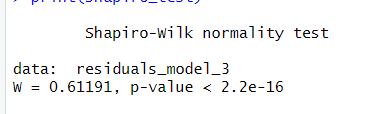
\includegraphics[width=0.7\linewidth]{graphics/5.5.6.png}
  \caption{Kiểm định Shapiro-Wilk mô hình 3 }
\end{figure}

Kết quả kiểm định Shapiro-Wilk cho mô hình 3:
\begin{itemize}
  \item\textbf{p-value < 0.05 }: Có bằng chứng bác bỏ H0.
  \item\textbf{Kết luận}: Phần dư không tuân theo phân phối chuẩn, giả định phân phối chuẩn bị vi phạm.
\end{itemize}

Dựa trên biểu đồ phân phồi phần dư:
\begin{figure}[H]
  \centering
  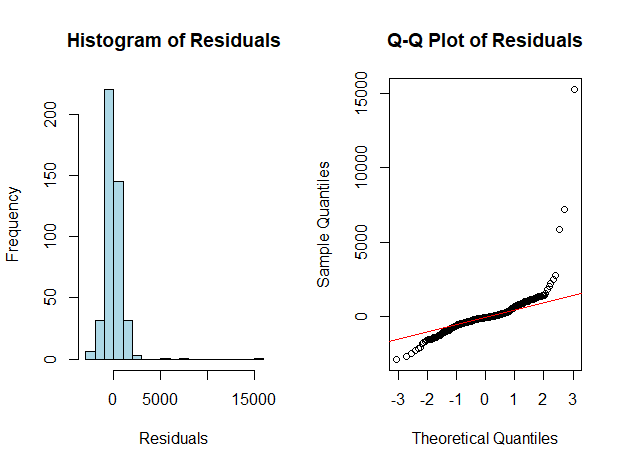
\includegraphics[width=0.5\linewidth]{graphics/5.5.9.png}
  \caption{Đồ thị phần dư ở mô hình 3}
\end{figure}

\begin{itemize}
  \item\textbf{Histogram of Residuals}: Biểu đồ histogram cho thấy phần dư không có dạng phân phối chuẩn. Phân phối phần dư bị lệch mạnh sang một phía (lệch phải), và không tuân theo dạng chuông đối xứng của phân phối chuẩn.
  \item\textbf{Q-Q Plot of Residuals}: Trong biểu đồ Q-Q plot, các điểm không nằm trên đường thẳng đỏ (đường kỳ vọng cho phân phối chuẩn), đặc biệt ở hai đầu (tail). Điều này chỉ ra rằng phần dư không tuân theo phân phối chuẩn.
  \item\textbf{Kết luận}: Cả hai biểu đồ đều hỗ trợ kết quả của kiểm định Shapiro-Wilk (p-value < 0.05), khẳng định rằng phần dư không tuân theo phân phối chuẩn.
\end{itemize}

Kiểm tra phương sai đồng nhất: Sử dụng biểu đồ Scale-Location và kiểm định Breusch-Pagan

Kiểm định Breusch-Pagan

Giả thuyết đặt ra:
\begin{itemize}
  \item\textbf{Giả thuyết H0}: Phương sai của sai số là đồng nhất (phương sai đồng nhất).
  \item\textbf{Giả thuyết H1}: Phương sai của sai số thay đổi (phương sai không đồng nhất).
  \item\textbf{Nếu p-value > 0.05}: Không có bằng chứng bác bỏ giả thuyết H0, phương sai đồng nhất.
  \item\textbf{Nếu p-value ≤ 0.05}: Bác bỏ H0, phương sai không đồng nhất.
\end{itemize}

\begin{figure}[!htp]
  \centering
  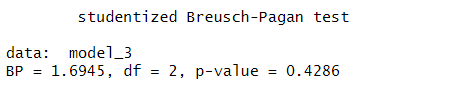
\includegraphics[width=0.5\linewidth]{graphics/5.5.10.png}
  \caption{Kết quả kiểm định Breusch-Pagan mô hình 3 }
\end{figure}

Dựa vào kết quả kiểm định Breusch-Pagan mô hình 3:
\begin{itemize}
\item\textbf{Với p-value = 0.4286 > 0.05}: chúng ta không có đủ bằng chứng để bác bỏ giả thuyết H₀. Điều này nghĩa là phương sai của sai số được xem là đồng nhất.
\item\textbf{Kết luận}: Dựa trên kiểm định Breusch-Pagan, mô hình không vi phạm giả định phương sai đồng nhất. Phương sai của phần dư ổn định và thích hợp với hồi quy tuyến tính.
\end{itemize}

Dựa vào biểu đồ Scale-Location:

\begin{figure}[H]
  \centering
  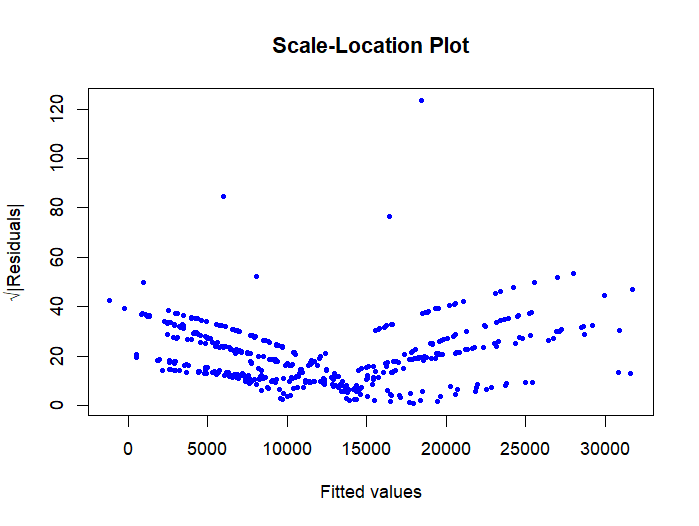
\includegraphics[width=0.5\linewidth]{graphics/5.5.11.png}
  \caption{Biểu đồ Scale-Location }
\end{figure}

\begin{itemize}
  \item\textbf{Nhận xét}: Các điểm không phân bố ngẫu nhiên xung quanh đường ngang (red line) mà có dạng hình phễu, tức là phương sai của phần dư không đồng nhất. Hiện tượng này cho thấy có thể vi phạm giả định đồng nhất phương sai, nghĩa là sai số của mô hình có sự thay đổi tùy thuộc vào giá trị dự đoán.
  \item\textbf{Kết luận}: Dựa trên kết quả kiểm định Breusch-Pagan, phương sai của phần dư trong mô hình 3 là đồng nhất.
  Tuy nhiên, biểu đồ Scale-Location vẫn gợi ý cần xem xét thêm.
\end{itemize}

Kiểm tra tính tuyến tính: sử dụng biểu đồ Residuals vs Fitted để kiểm tra:

\begin{figure}[H]
  \centering
  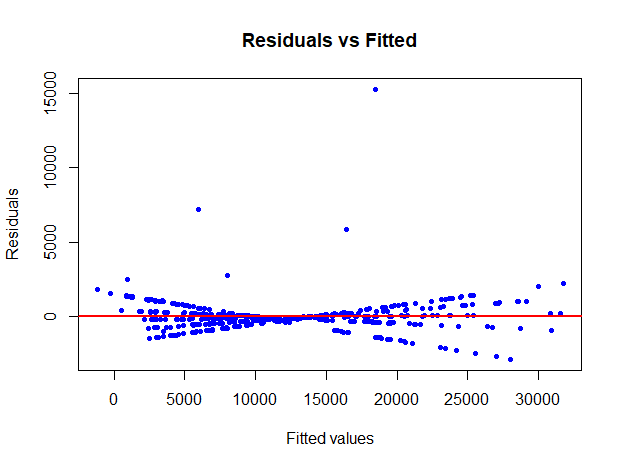
\includegraphics[width=0.5\linewidth]{graphics/5.5.12.png}
  \caption{Biểu đồ Residuals vs Fitted của mô hình 3 }
\end{figure}
\begin{itemize}
\item\textbf{Nhận xét }: Phần dư không phân bố ngẫu nhiên quanh đường ngang tại Residual = 0: Có một dạng hình quạt, nghĩa là ở các giá trị dự đoán thấp và cao, phần dư có xu hướng biến động mạnh hơn.
\item\textbf{Kết luận}: Không đảm bảo tuyến tính, dạng hình quạt của phần dư gợi ý rằng mối quan hệ giữa biến phụ thuộc và biến độc lập không hoàn toàn tuyến tính.
\end{itemize}


Kiểm định độc lập sai số : để kiểm tra độc lập của sai số trong mô hình hồi quy, sử dụng kiểm định Durbin-Watson trong R. Kiểm định này kiểm tra xem có tự tương quan bậc nhất trong phần dư hay không. Nếu giá trị Durbin-Watson gần 2, giả định độc lập của sai số được thỏa mãn.

Giả thuyết kiểm định Durbin-Watson
\begin{itemize}
  \item\textbf{Giả thuyết H0}: Sai số không có tự tương quan.
  \item\textbf{Giả thuyết H1}: Sai số có tự tương qua bậc nhất.
\end{itemize}

\begin{figure}[H]
  \centering
  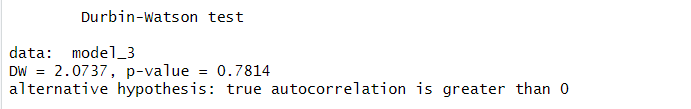
\includegraphics[width=0.5\linewidth]{graphics/5.5.8.png}
  \caption{Kiểm định Durbin-Watson của mô hình 3 }
\end{figure}

Kết quả kiểm định Durbin-Watson cho mô hình 3:
\begin{itemize}
  \item\textbf{Giá trị Durbin-Watson (DW)}: 2.0737(gần 2) cho thấy rằng không có tự tương quan bậc nhất đáng kể giữa các phần dư (residuals). Điều này thỏa mãn giả định độc lập của sai số.
  \item \textbf{p-value}: 0.7814(lớn hơn mức ý nghĩa 0.05) chỉ ra rằng không có bằng chứng thống kê để bác bỏ giả thuyết H0, tức là không có hiện tượng tự tương quan dương trong phần dư.
  \item\textbf{Kết luận}:  Mô hình 3 đảm bảo giả định độc lập của sai số, và kết quả hồi quy có thể được sử dụng một cách tin cậy liên quan đến giả định này.
\end{itemize}

\subsubsection{Kết luận}

Mô hình 3 có độ phù hợp tương đối tốt với dữ liệu, với \textbf{R-squared} cao và các biến độc lập có ý nghĩa thống kê.

Đồ thị chẩn đoán cho thấy một số vấn đề tiềm ẩn về tuyến tính, phương sai đồng nhất và phân phối chuẩn của phần dư. Mặc dù có một số điểm cần lưu ý, nhưng chúng không quá nghiêm trọng.

Có thể kết luận rằng mô hình 3 tương đối đúng và phù hợp để dự đoán \textbf{order\_total}. Tuy nhiên, cần kiểm tra thêm và có thể thực hiện một số điều chỉnh nhỏ để cải thiện thêm độ chính xác của mô hình.







